\section*{Cloud setup}

For our cloud setup, we used Docker \cite{docker} containers running in a DigitalOcean \cite{do} instance (Figure~\ref{fig:do}).
We decided to install ElasticSearch \cite{es}, a RESTful search and analytics database that works well with its dashboard builder, Kibana \cite{kibana}.
The setup was relatively straightforward, but we had some troubles at first because we discovered ElasticSearch is a quite memory-intensive program, therefore we had to resize our cloud instance to have more RAM available, as well as research how to allocate more memory for Docker containers. \\ \\
\begin{figure}[H]
    \centering
    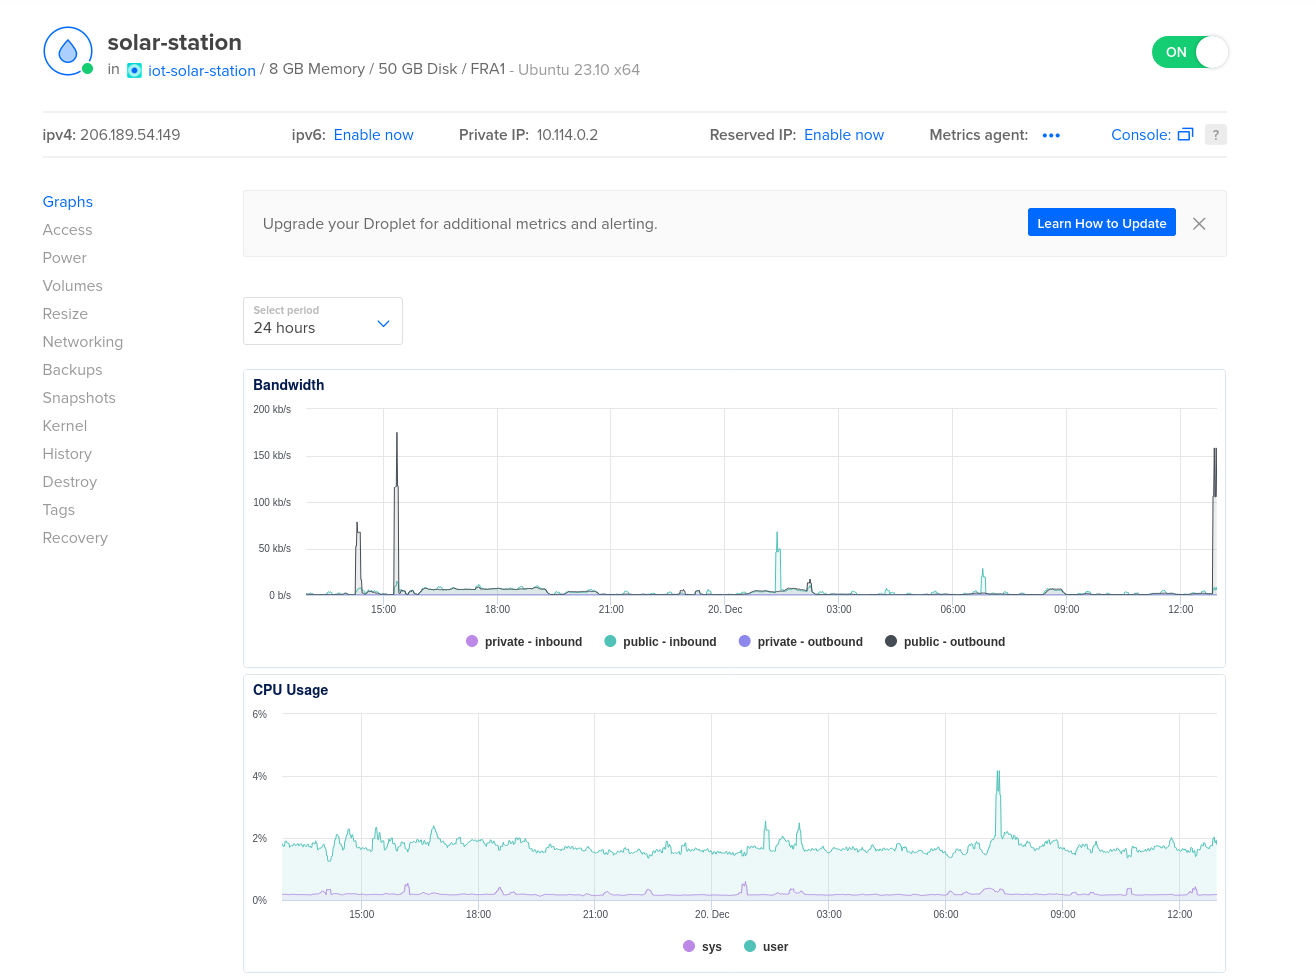
\includegraphics[width=\textwidth]{../assets/png/digital-ocean-graph}
    \caption{A sneak peek of the DigitalOcean interface showing some telemetry about our cloud instance.}
    \label{fig:do}
\end{figure}\
This allowed us to develop faster in the end because we had a shared database for measurement.
We could collaborate more easily asynchronously as we had the same development environment for everyone.
It is also a more realistic setup, although no HTTPS certificate was installed.
We also had to specify the necessary port-forwarding rules in the intuitive DigitalOcean web interface to allow outside connection. \\ \\
A list of the steps undertaken for this part can be found in file \texttt{scripts/es\_setup.sh} in the delivered zip.

\begin{figure}[H]
    \centering
    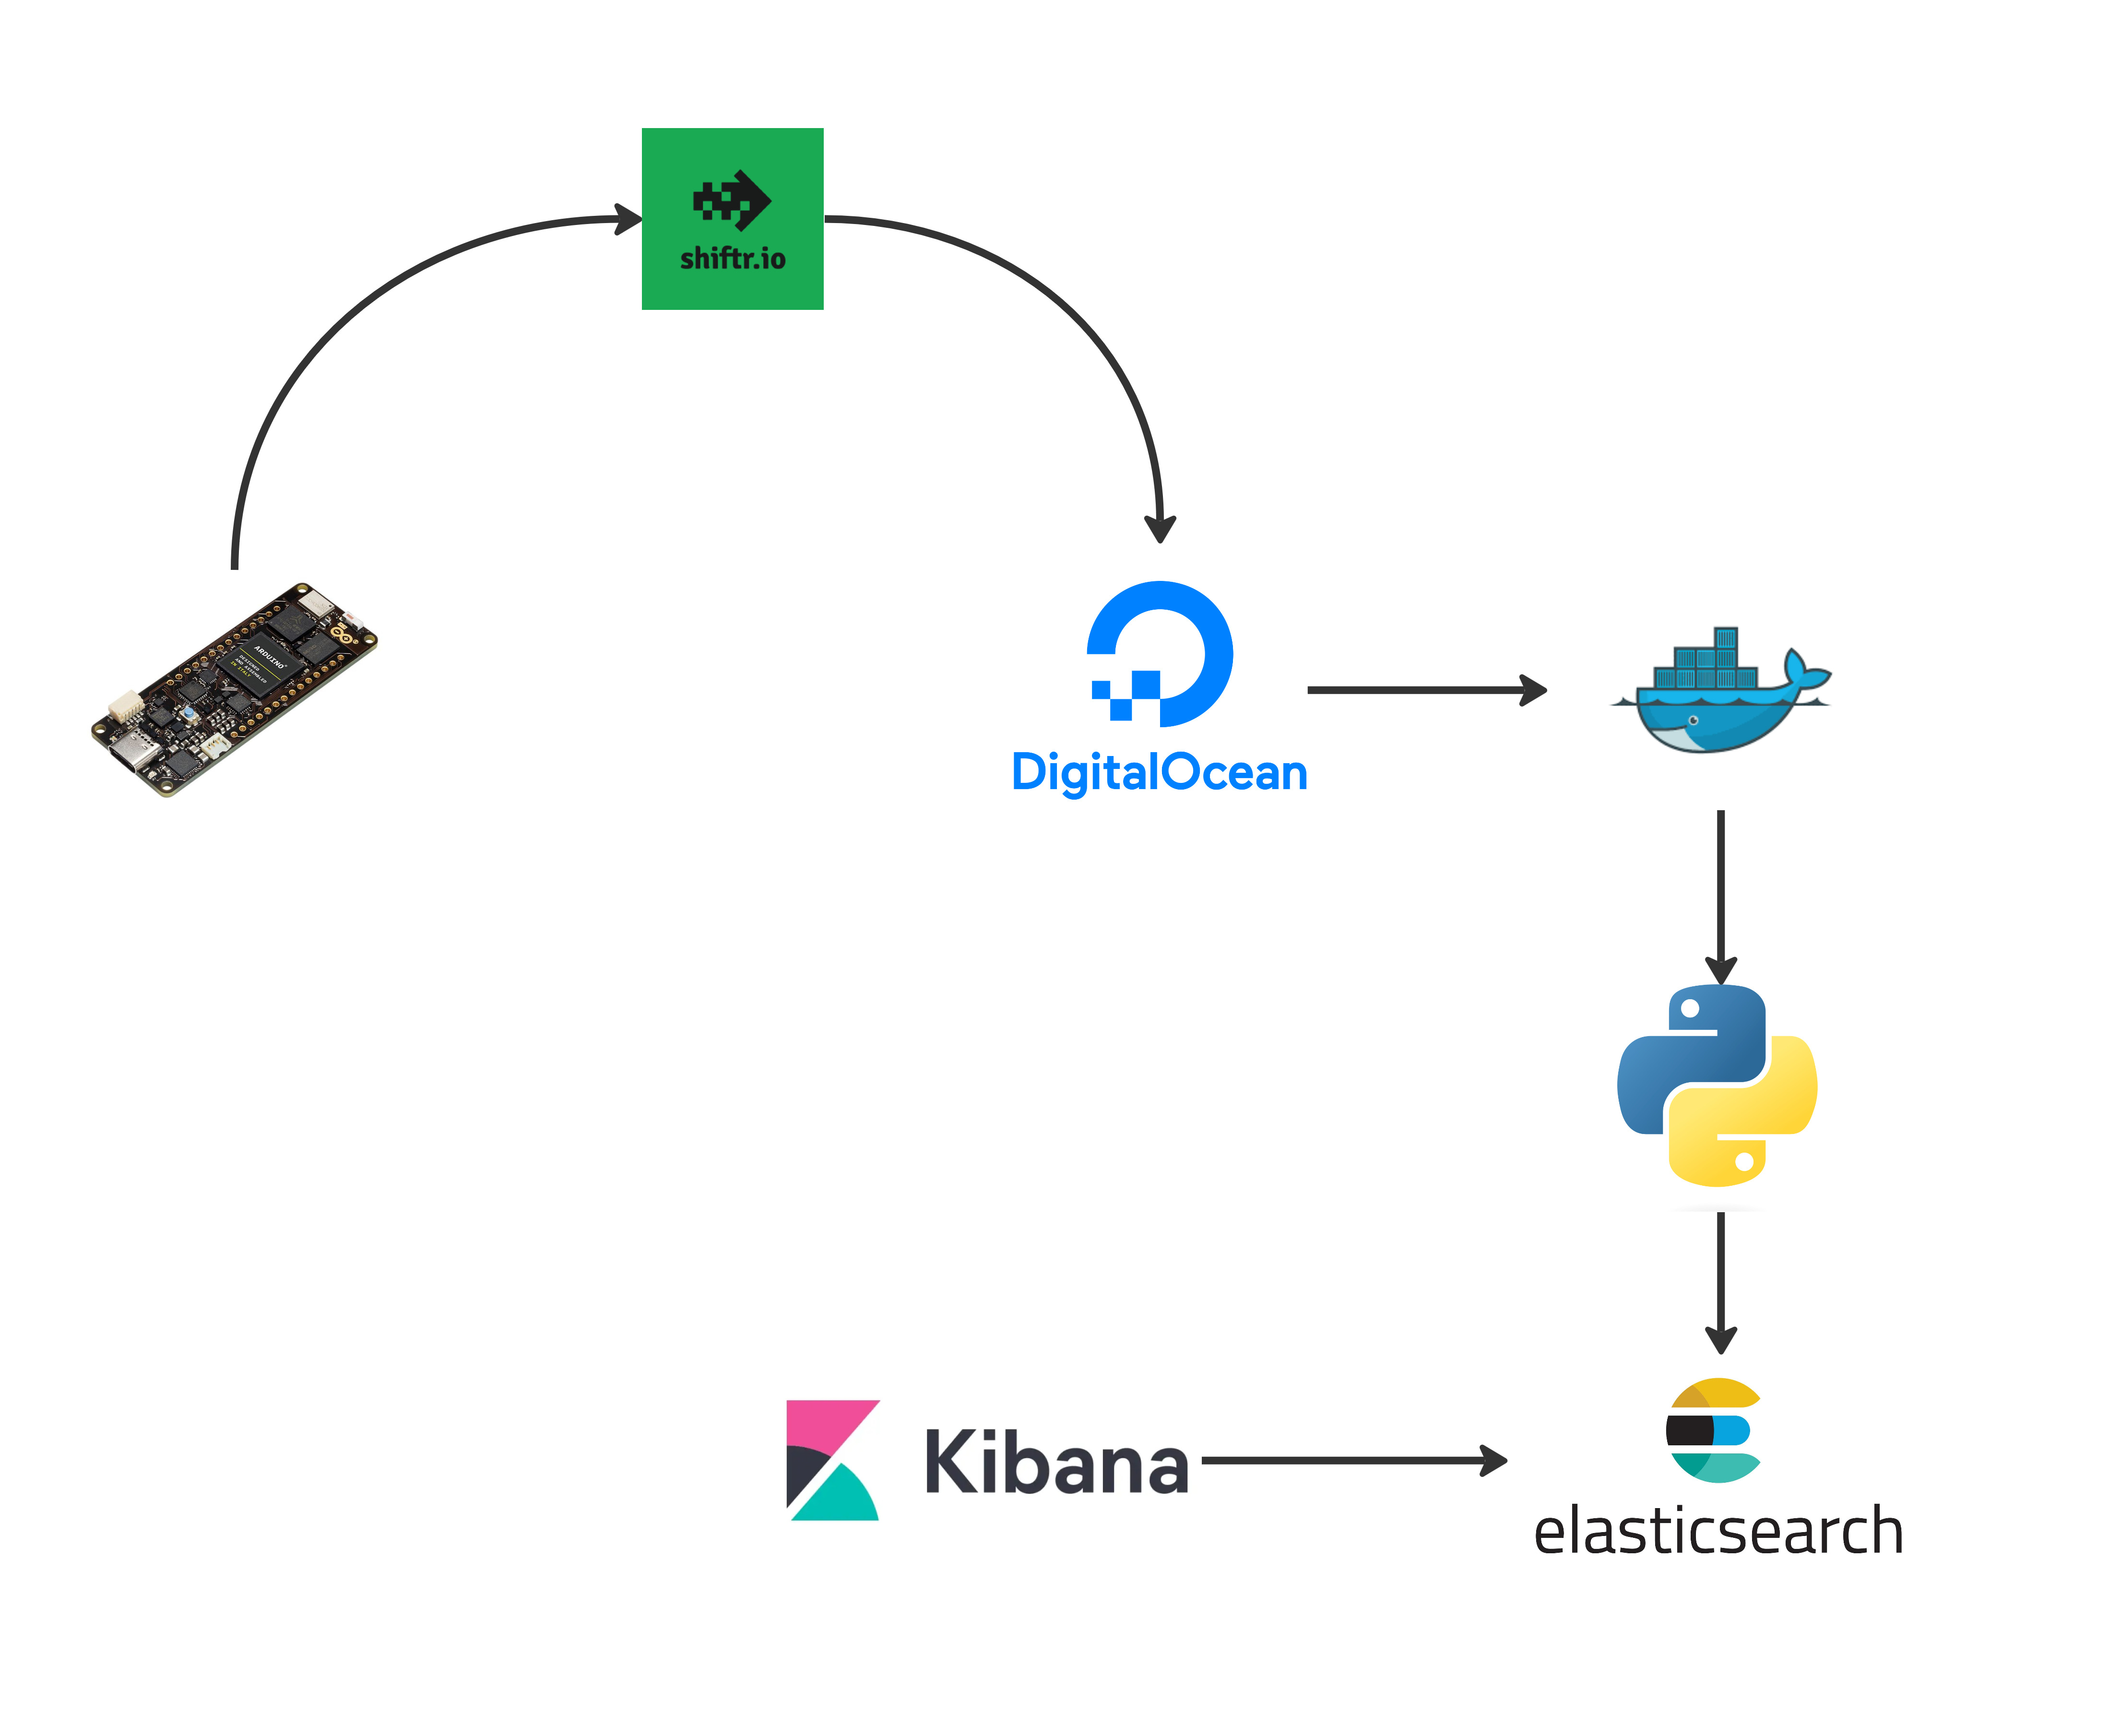
\includegraphics[width=\textwidth]{../assets/png/solar-station-arch}
    \caption{A simple diagram showing the deployment architecture of our application.}
    \label{fig:do}
\end{figure}\